% status: 100
% chapter: Application


\def\paperstatus{100} % a number from 0-100 indicating your status. 100
                % means completed
\def\paperchapter{Application} % This section is typically a single keyword. from
                   % a small list. Consult with theinstructors about
                   % yours. They typically fill it out once your first
                   % text has been reviewed.
\def\hid{hid-sp18-hid524} % all hids of the authors of this
                                % paper. The paper must only be in one
                                % authors directory and all other
                                % authors contribute to it in that
                                % directory. That authors hid must be
                                % listed first
\def\volume{9} % the volume of the proceedings in which this paper is to
           % be included

\def\locator{\hid, Volume: \volume, Chapter: \paperchapter, Status: \paperstatus. \newline}

\title{Report: Big Data in Healthcare}

\author{Hao Tian}
\affiliation{%
  \institution{Indiana University}
  \streetaddress{School of Informatics, Computing and Engineering}
  \city{Bloomington} 
  \state{IN} 
  \postcode{47408}
  \country{USA}}
\email{tian4@indiana.edu}


% The default list of authors is too long for headers}
\renewcommand{\shortauthors}{H. Tian.}


\begin{abstract}
Health, as the most important factor that influences 
the happiness with life, 
people pay great attention and put much effort into it. 
The term ``healthcare'' is the 
result of efforts to maintain a healthy condition in the 
general public. 
However, the growing population brings many challenges to 
the healthcare field. To provide people with a good  
healthcare environment, the traditional healthcare field 
needs to cooperate with 
cutting-edge technologies in order to fit the population. 

Healthcare today is an important topic throughout the world, and as 
the population is growing, human health needs 
to be protected by more advanced methods and technology. For tracking 
health in the population, each country needs a complete medical 
care system, which could monitor general health conditions and offer 
valuable information to medical services, such as 
hospitals, disease research institutions, and even national security agencies. 
However, as the population stands now, the traditional 
methods and technologies cannot fully support the requirement to
satisfy the healthcare needs for most people.

To satisfy the entire population's healthcare needs with a functioning 
healthcare system, the cutting edge technology concepts - Big Data - 
provide the tools needed to develop better healthcare systems. 
The basic concept of Big Data is to process and analyze a large amount 
of data, including data mining, data visualization, and using machine 
learning knowledge to predict  future situations. With the large amount of 
data needing processing in the healthcare fields, using the knowledge for 
processing massive amount of data is very helpful in dealing with 
issues that healthcare systems are facing today. 

This paper discusses the Big Data technologies and applications that 
are currently being used in healthcare fields, and the possible technologies 
that might be used in the future in order to improve the quality of health 
care. The serious illnesses, such as cancers, AIDS and other deadly 
diseases, are also included in the discussion about the technologies 
concerned with healthcare. 
\end{abstract} 

\keywords{\locator\ Big Data, healthcare, Medical Care, 
Data Mining, Cancer.}

\maketitle

\section{Introduction}
\subsection{Healthcare}
In starting this paper, we need to define what healthcare is. According 
to the definition from the Merriam Webster dictionary: healthcare is an 
effort to maintain people in a healthy condition using treatment given by 
trained and licensed medical professionals~\cite{def_hc}. 
The healthy condition indicates that both 
physical and mental status are healthy, and they are basic 
factors that lead people to live a happy life. 

Each country in the world has different healthcare systems to 
maintain citizens' health and protect citizens from getting diseases. 
The countries like Canada, the United Kingdom, and China have 
uniform healthcare systems, like national healthcare services 
provided to all the citizens~\cite{ca_hc, uk_hc, cn_hc}. The 
United States of America, as a developed country, has a very unique 
status regarding healthcare: the U.S. does not have a uniform healthcare 
system and had no universal healthcare coverage for U.S. citizens until 
2016~\cite{us_hc}. The free market for medical care in the U.S. brought 
great value to the U.S. economy~\cite{us_hccost}, but the lack of 
government management has caused trouble accessing health care 
for some people~\cite{us_hcs}.

\subsection{Big Data}
Since the start of the second decade in the twenty-first century, 
the amount of information that people see and read each day has 
grown to be much higher that before, 
and the traditional methods and technologies for data processing are 
inadequate for this period of dramatically growing data 
sizes~\cite{Moura}. In this situation, people have realized the 
significance of developing more advanced data processing methods 
and technologies. 

Big data is a term referring to the technologies that are used to 
process large amounts of data, and it is also a major concept 
used in the future technologies. The word 
``Big Data'' has been given three characters. 
It has also been called 3 Vs~\cite{3v}:
\begin{itemize}
	\item Variety: the categories of data are more varied; the data could be in 
	different forms, such as videos, sounds, and texts. Today, data processing 
	techniques should be able to gain information from different types of 
	data.
	\item Velocity: the speed of data processing has become more demanding; 
	people need more efficient ways to collect data or process data. 
	``Real-time'' indicates the immediate updating of data.
	\item Volume: data size is incredibly big, the traditional computation 
	methods will be abandoned because they cannot handle it. 
	More efficient methods or applications need to be created.
\end{itemize}

The future technologies need to fit the rapidly increasing pool of
data, and the data size is still growing. More than traditional data 
processing, such as data cleaning, and raw data processing to 
convert unreadable data into data that humans can read, the 
data size of today also brings 
another opportunity for people to gain valuable information from the data. 
Indeed, the Big Data-related technologies have more jobs available than the 
traditional technologies; analyzing data and predicting outcomes 
from data become 
very important parts of the Big Data idea. Despite the fact that analysis
and prediction are not new, the growing amount of data enhances the 
importance of those theoretical concepts from mathematics and 
statistics~\cite{Moura}.

\subsection{Healthcare and Big Data}
Today, the human population on earth is 7.6 billion~\cite{p2018_1}, and 
most of the population is concentrated in Asia, in countries such as 
China, India, and 
Southeast Asian countries~\cite{p2018_2}. Each person 
could be seen as a dataset with different variables concerned with health 
conditions, and the whole world is a huge, unformatted database, which 
includes all of that datasets. For each healthcare system, whether 
it contains public 
healthcare systems or private healthcare companies, this amount of data 
challenges every healthcare organization, and they need to develop 
adequate methodologies and use advanced technologies to achieve the 
purpose of helping people to maintain good health.

Big Data concepts have been implemented in many fields, including the 
healthcare area. The Big Data-related technologies, such as real-time 
data analysis, cloud computing, and data visualization, cut the cost of 
traditional data processing methods, which brings efficiency to the health 
care area and also lowers the cost compared to the traditional healthcare 
field~\cite{intro_hb1}. 

\subsection{Paper Layout}
The paper is organized according to the following structure: 
\begin{enumerate}
	\item The beginning of the paper discusses the trends within the 
	healthcare field,
	 as well as how the Big Data concepts and technologies affect the 
	 traditional healthcare field. 
	\item Then the paper talks about the elementary component of the 
	current healthcare industry, the data. The data transformation 
	from paper to digital is the key to apply the newest technologies 
	to the healthcare field, and 
	it is also one of the major obstacles that limits the evolution of the
	 healthcare field. 
	\item The Internet of Things technology (IoT) is a great application in 
	today's healthcare industry, because it provides real-time data to 
	healthcare systems, and it also makes the healthcare service 
	more efficient, despite the fact that it is not perfect.
	\item The cloud computing infrastructure of the common 
	healthcare systems that combine 
	the Big Data technologies is an important part of today's healthcare 
	industry. 
	Because of the distribution system infrastructure used in the healthcare
	field, today's healthcare services can process a large amount of data and 
	serve numerous patients at the same time.
	\item After discussing those important technologies used in the 
	healthcare 
	field, the paper talks about the healthcare services that are used today.
	The important aspects in the healthcare field will be discussed, 
	such as data analysis of digital medical data, gene prediction 
	on potential health threats,
	and powerful systems that are used for healthcare services.
	\item After all the discussions about technology, the paper 
	starts to put forth a new 
	perspective: the healthcare in the future. In this section, 
	the paper discusses new thoughts and 
	new technologies that might be used in the future in order to make the 
	healthcare services better.
	\item Summary of the paper.
	
\end{enumerate}


\section{Trends in healthcare today}
The growing population has become a challenge for the traditional healthcare 
area, but as the amount of data grows, it also brings numerous 
opportunities for the health 
care area to provide better services. As time goes by, the healthcare area 
has made many improvements and has also improved its methods and 
technologies. Carol McDonald, an experienced medical and 
health insurance-related application developer, mentions some trends 
showing how Big Data is changing the healthcare area, which could 
be summarized as three major changes~\cite{5trends}:
\begin{itemize}
	\item \textbf{Data:} In the healthcare field, the data quality 
	will be better 
	in its relevance and accuracy in the future. In order to 
	provide better health 
	care services, the information about each patient 
	will be more closely 
	related to the important factors that go into health 
	condition 
	evaluation~\cite{hdata}. More crucial data will be 
	included in the database, 
	and the size of false data is decreasing~\cite{hdata}.
	\item \textbf{Methods:} The ``methods'' here indicate 
	the theoretical 
	statistical and theoretical mathematical methods that 
	have been used in 
	healthcare to 
	provide data analysis services. As the date size is 
	growing each day, the 
	opportunity has come to many fields. The growing 
	data brings the 
	healthcare companies a great chance to improve 
	healthcare service 
	quality by offering patient healthcare plans. 
	Healthcare companies could 
	use statistical, mathematical and artificial 
	intelligence knowledge to help 
	patients to make plans about their healthcare investments.
	\item \textbf{Technologies:} The clinical service is improving, 
	and more and more advanced technologies have been used in 
	hospital, medical care and 
	elder care settings. This trend helps improve 
	technologies in health 
	care. One of the most classic examples is the 
	usage of IoT (Internet of 
	Things) in healthcare~\cite{iot}; the medical devices such as real-time 
	medical monitors and trackers could update 
	the health data 
on patients, which is a efficient method for 
providing more rational health 
	services, even if it somehow 
	compromises the privacy slightly.
\end{itemize}

\section{Data in healthcare}
The digital data growth in healthcare is remarkable: according to the Dell 
EMC Digital Universe research team, the digital data in 
the healthcare field is 
4.4 zettabytes, with a 40 percent growth rate annually~\cite{EMC2015}. 
Compared with other fields, healthcare is one of the fastest growing 
segments in digital data in the world, and the healthcare applications 
are pushing the growth even more~\cite{EMC2015}. 

Despite the fact that the data growth in the healthcare field brings 
information to healthcare 
companies, the data quality is not guaranteed because of data format 
and source issues. Especially for the medical data, because medical 
data is so complex (due to concerns about scale of data dimension, 
missing values in databases, biased data and so on); even slight 
inconsistency in the databases could require much time and 
effort to fix~\cite{Lee2017}. However, 
people have come up with various solutions for improving the 
overall quality of data that would be used in the healthcare industry.

\subsection{EHR - Electronic Health Records}
Electronic Health Records (ERC) is the name for digital 
health condition data, and 
it stores patient health data~\cite{EHR}. Storing the 
digital data of each 
patient is a basic concept that exemplifies applying Big Data
 ideas into healthcare, 
since digital data is the foundation of applying data analysis, data 
machines, and machine learning methods and technologies. 
Figure 1 shows 
how the EHR collaborates with other segments of healthcare 
systems~\cite{Reddy2013}.
 
\begin{figure}[!ht]
\centering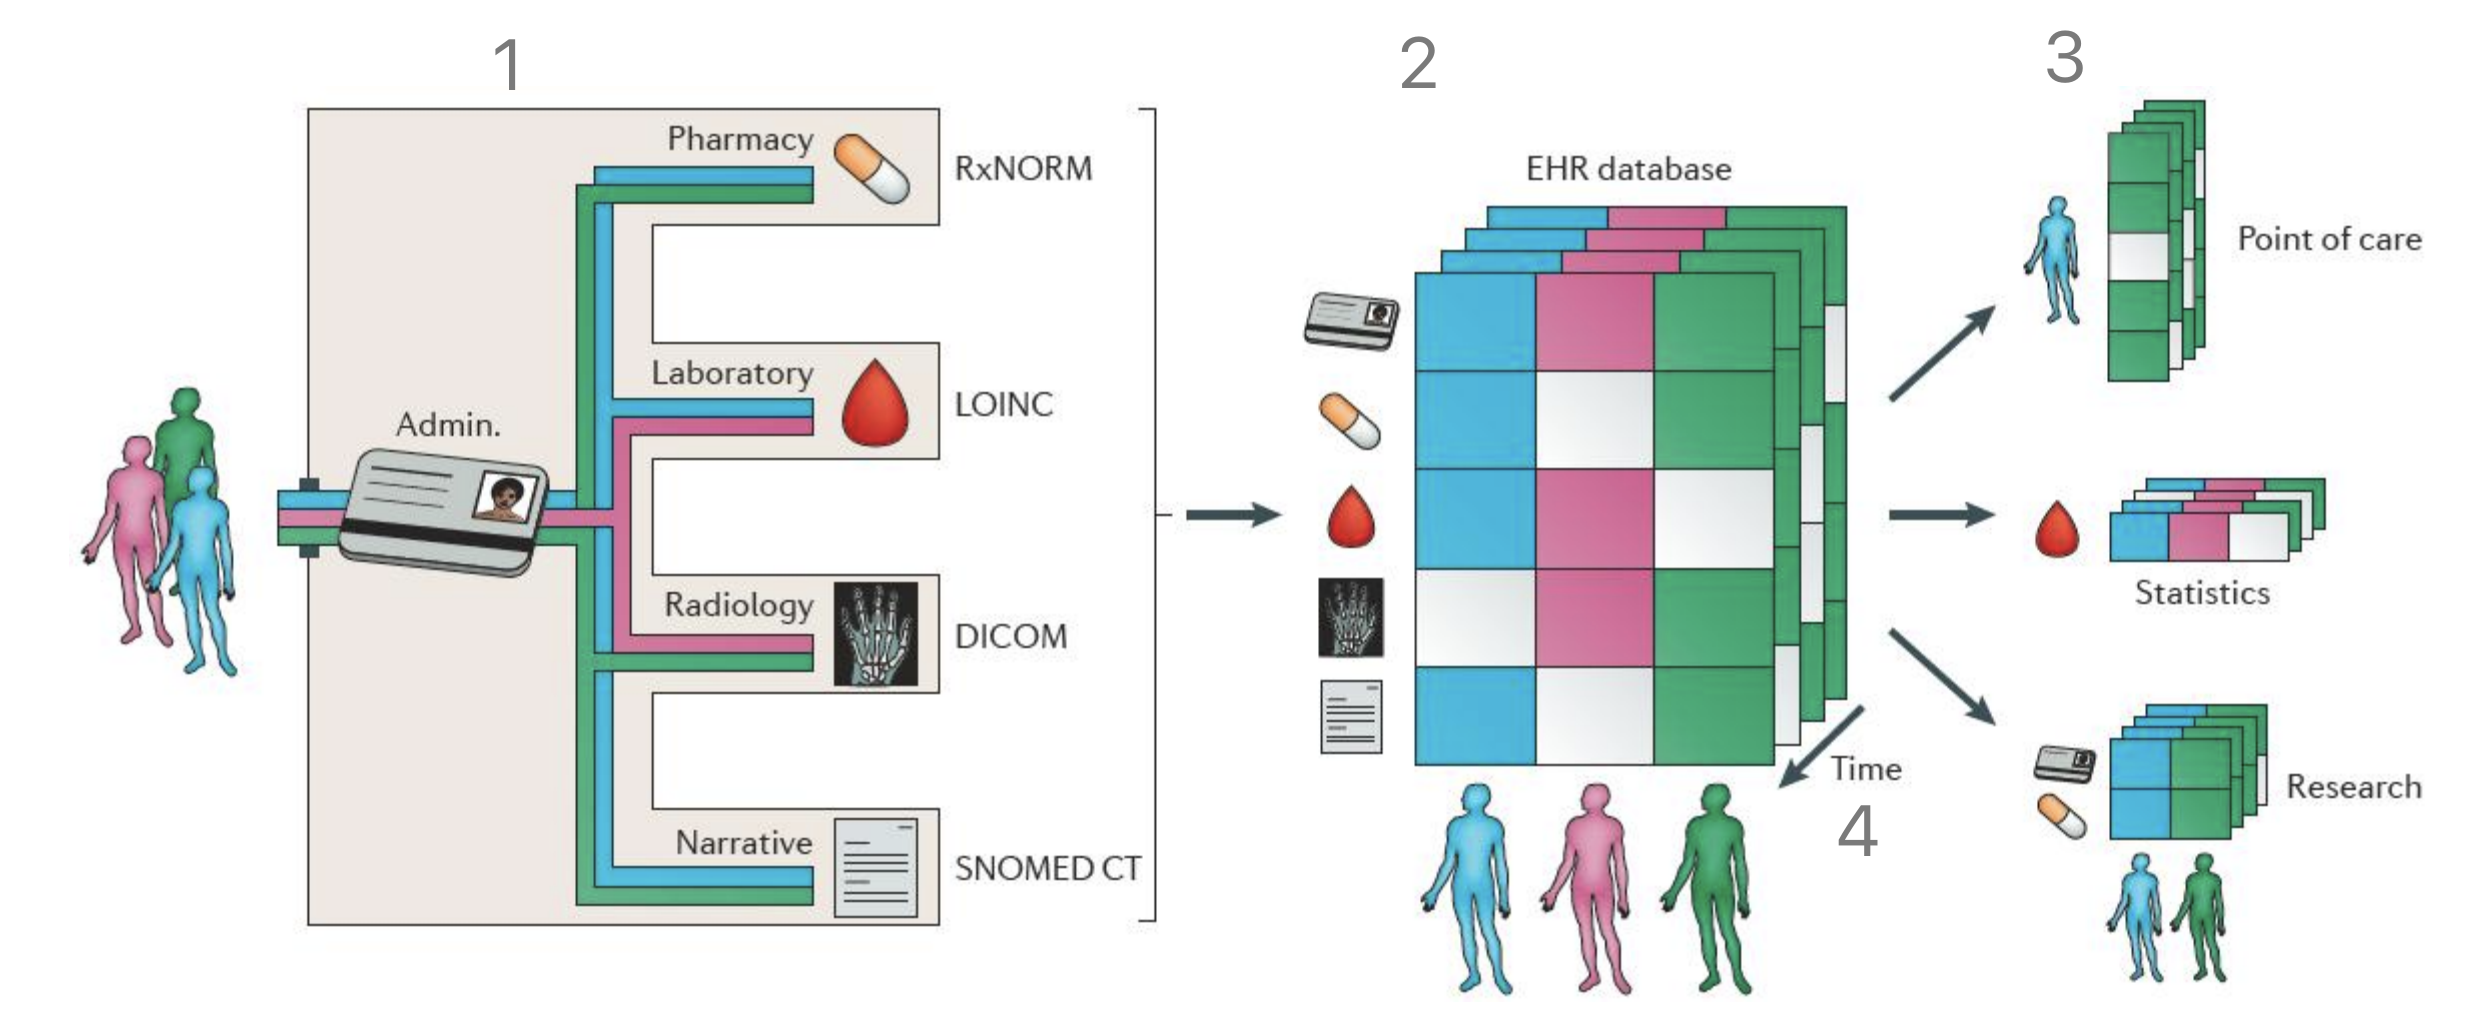
\includegraphics[width=\columnwidth]{images/EHR.png}
\caption{How does a classic EHR system work}\label{f:EHR}
\end{figure}

Figure 1 shows a stream chart showing how a classic EHR system works. In 
general, it could be separated into four components (each component's 
order numbers follow the number in Figure 1)~\cite{EHR}:
\begin{enumerate}
	\item First, patients provide their health data in a certain format,
	 and the format depends on the EHR system. The components include 
	 different types of information, and each type of 
	 information will be used for 
	 different purposes.
	\item The EHR database collects all the data. 
	The data will be stored for 
	future usage.
	\item Base on the need the patient has, the EHR system 
	uses appropriate data 
	for different needs. Some EHR systems need human 
	support for making 
	plans and managing the healthcare for patients, 
	but some systems do not 
	need human support, depending on the design 
	and implementation of 
	the system.
	\item Patients get their results from the system.
\end{enumerate}

In the United States, the United Kingdom, and other developed countries in 
Europe, 
the EHR systems have been put into wide use in hospitals, research 
institutions, and healthcare companies~\cite{Ross2014}. The EHR database 
can be shared by the patients, healthcare providers, and others who have 
permission to access the data on certain patients~\cite{Reddy2013}. The 
EHR data that is open to the public (including non-sensitive
 information regarding
patients) could be used as the material for multi-purpose studies on public 
disease distribution, making healthcare plans and decisions for patients, and 
also predicting future circumstances regarding health 
conditions in certain patients 
or the general public~\cite{Ross2014}. 

Despite the fact that EHR systems have been widely used by 
many countries and many 
organizations, because of the natural complexity of the medical data, the 
EHR has limited ability to pre-process and 
analyze it~\cite{Ross2014}. Although EHR systems have been 
implemented by 
many healthcare institutions in the United States, even today, 
the United States 
does not have a uniform EHR system; the constraints of local EHR 
databases cannot provide the qualified data analysis. 
Furthermore, because different institutions use different 
EHR systems, the connections between 
them cannot form a uniform system, which could provide a more powerful 
healthcare system for the country. More than that, the privacy of the EHR 
data is also a controversial topic; many patients refuse to 
publish their health data due to privacy concerns, which is a 
non-negligible problem, because some of the information is crucial for 
certain data analysis jobs~\cite{Ross2014}.

\subsection{KP HealthConnect - A successful EHR system}
KP HealthConnect is a successful EHR system model developed by Kaiser 
Permanente. Kaiser Permanente is a massive healthcare company 
founded in California, U.S., and KP HealthConnect 
exemplifies a successful pattern 
of EHR system use~\cite{kp1}. KP HealthConnect covers 
some states in the U.S. 
(most of them are on the West Coast), and the feedback from both patients 
and physicians sides is quite positive~\cite{kp1}.

Just like how the general EHR system works (Section 3.1), 
the KP healthcare 
needs patients to provide their EHR data to the system first, then physicians 
or medical specialists, and the system itself, 
will process the data for analysis
and deep learning, but why could KP HealthConnect be called 
``a complete EHR system'' 
with high evaluation scores from users? According to the 
study from The Commonwealth Fund (a healthcare company), the key 
components of  KP HealthConnect's success are as 
follows~\cite{McCarthy2009}:
\begin{itemize}
	\item \textbf{Lowers the communication cost:} Compared with other 
	EHR systems, KP HealthConnect lowers the communication 
	cost between 
	patient and doctors. Patients can fill online surveys to report their 
	health conditions without communicating with their doctors or health 
	care providers ordinarily. 
	\item \textbf{Provides more access to patients:} the system provides 
	patients with more privileges to manage their 
	own data in the EHR system; 
	they can choose the data that they would like to provide 
	to the system, 
	to doctors, or to the public. 
	\item \textbf{Learning Models:} The EHR data in the system could be 
	used for providing patients with the future healthcare plans. The study 
	model in the KP HealthConnect system can use the 
	data that patients provide 
	and the medical knowledge in the model to create a special health 
	plan for each patient. 
\end{itemize}
Indeed, the KP HealthConnect is a great EHR 
system that only needs slight
human assistance for the system to work, 
but the system only covers fewer
than ten states in the United States, so the EHR 
database is not large enough for 
the learning models to come up with rational decisions. 
More than the size 
of the EHR database, KP HealthConnect still has issues 
with data consistency: 
the databases in different data centers could be different, 
and it is usually caused by delayed data 
updating~\cite{Suarez2013}. The 
issue indicates that the distribution system in KP HealthConnect is 
not well formed or implemented. 

\subsection{Cancer Biomedical Informatics Grid}
Cancer has became one of the 
most lethal diseases in the world, and there are no treatments 
proven to cure cancer. Even today, people are still short on knowledge 
about it, 
and the trend of today is that more and more people are getting cancer. 
In order to 
gather information about cancer for the purposes of learning about 
cancer and preventing cancer from occurring, the National Cancer 
Institute (NCI) developed the 
Cancer Biomedical Informatics Grid (caBIG)~\cite{Califano}.

The caBIG is a clinic database and system used for cancer study; 
specifically, scientists and medical specialists from the NCI use the 
data collected from different resources to study cancer. The 
infrastructure of the caBIG system allows scientists and 
medical specialists to study the data 
and use the applications offered by the system to conduct studies 
concerned with predicting cancer growth, forming patient treatment plans, 
and communicating data and study results~\cite{Califano}. The caBIG 
is a great step for people to fight against cancer by gathering 
information and concatenating 
data, systems, and scientific professional resources together to study it.

However, in reality, the outcomes of the research conducted by 
using caBIG 
database and system are not optimal, due to many 
reasons~\cite{Califano}:
\begin{itemize}
	\item The infrastructure of the caBIG system is too complicated because 
	of the nature of data needed for cancer studies. Additionally, 
	funding the system 
	is too expensive. Most of the money is not used in the laboratory; 
	instead, most of the cost has been used to build the heavy 
	load database and the 
	program management, because the contents in the caBIG system are too
	complex and the communication between the research community and the 
	system leader is not efficient.
	\item Since the NCI is a life science institution, the actual coding program 
	implementation of the caBIG is not NCI. NCI sells the job out to some 
	technicians to complete it as contractors. However, the contractors 
	building the project do not really understand cancer research. The project 
	does not actually meet the requirements for the research.
	\item The commercial usage of the caBIG is unsustainable, since the 
	complexity of the system restrains the research, and it also limits the 
	actual services that NCI could provide to the public and all potential 
	users, even though the caBIG is free and open source.
	\item Because of the complexity of the caBIG system, poor 
	communication between technicians and researchers, and the 
	slow pace at which the research happens, 
	the caBIG system leader layer does not have a goal that matches 
	the purpose of using the caBIG. 
	Instead, the caBIG becomes a huge, sophisticated data collection device
	that has little functional value.
\end{itemize}
Despite that in reality, the caBIG does not provide desirable results to the 
public, it is undeniable that caBIG represents a valiant attempt in 
building a massive database system to fight against cancer. 

\subsection{Limitation of healthcare Data today}
Even though the digital health data has become more common 
in practice, the issues and the potential risks still exist in the 
data. From the general EHR 
system for all diseases, and the caBIG for the cancer 
specifically, the healthcare data is always complicated, 
huge in memory, and lacking in
structured data. According to Dan LeSueur, a experienced technician in 
the healthcare industry, there are several difficulties the healthcare 
industry encounters in using the data~\cite{LeSueur}:
\begin{itemize}
	\item The healthcare data is complex, and each data owner has a 
	different form of data storage. The complex nature of healthcare
	 data is the numerous dimensions recorded for each patient's data, 
	 and as more and more 
	 patient data has been added to a database, the time complexity 
	 of exploiting the database has become harder and harder.
	\item The healthcare data is too widely distributed in different 
	places: different 
	hospitals, healthcare providers, and even doctors hold various 
	data about 
	patients, as well as information about diseases from different 
	places. The difficulty 
	about distributed data is more than geographic, but more 
	about the fact that the source 
	of the data is distributed by different sources.
	\item Data in the healthcare industry is not formatted; there 
	are too many 
	unstructured data pieces that do not fit in the structured 
	databases. According 
	to the experiences from EHR system implementations within all different 
	organizations, the unstructured data is a significant obstacle to the future 
	data analysis. Even the high-performing EHR systems, like KP 
	HealthConnect, cannot provide good learning results from unformatted 
	data collections.
	\item The inconsonance of definitions and standards about the data 
	influences the treatments. To be more specific, for example, different 
	doctors have different standards about a criterion: some level of the 
	criterion can be seen as the clue to a certain disease, but doctors might 
	disagree with that. Furthermore, the standards concerned with health 
	care and disease are always changing, and the new observations of 
	those standards cannot always be updated and published, which poses
	more obstacles to building healthcare applications.
	\item Missing data is a big issue in the healthcare data. It is usually 
	caused by the privacy concerns from the data providers; the 
	sensitive data is not usually provided by the patients, or the sensitive 
	data is not published to the public, although some of that sensitive data 
	is crucial for the data analysis~\cite{Ross2014}.
\end{itemize}
Given the current quality of the healthcare data, it is known that the process 
of improving the healthcare data quality is a long term project. Additionally, 
as the life science knowledge is improving, the data that will be used in the 
healthcare industry will be more complex.

\subsection{Public-Key Cryptography for Security of the Health data}
In previous sections, it is known that the privacy of the data is one of 
the major concerns that prevents people from offering complete 
health data records, 
since the sensitive information always appears in the health data. 
More than sensitive information, 
the IoT (Internet of Things) devices for health 
care also have the probability of being attacked by 
adversaries (for example, 
the Fitbit in Section 5.3.).

Although, as the emergence of internet technologies 
has enabled people to 
share information with each other, in the healthcare field, 
people can now have 
more access to their personal health data, and they can 
more easily share 
it with other people. As this situation appears, 
the security demand with 
the privacy of health data has become inevitable. 
For this demand, applying 
public-key cryptography methods could be a 
great practice for protecting the 
privacy of the healthcare data~\cite{pke}.

Public-key cryptography is one of the greatest inventions in the history 
of mathematics. By using two math-related keys (public key and private key), 
it makes it more secure to encrypt data, since only the private key can 
decrypt the data that is encrypted by using the paired public key. The 
security of public-key encryption makes it a good candidate for 
securing personal health data~\cite{pke}.

The more detailed process as to how the public-key encryption can be 
used is as follows: 
\begin{itemize}
	\item Every patient that goes to a hospital can have his/her own private 
	key, and then a public key is generated based on that private key. The 
	private key will be kept secure by the patient. 
	\item After the patient goes to the hospital, the new medical data will be 
	generated by the hospital, and then that data will be encrypted using the 
	patient’s public key. Then it can be stored in the hospital data system. 
	\item Whenever a doctor feels he needs to have access to that
	medical data, he can reach out to the patient again, and the patient can 
	use the private key to decrypt that medical data. 
\end{itemize}

The usage of public-key cryptography can not only work
 in a hospital data 
system, but it can also work whenever people are going 
through an activity 
that generates the personal health data. For example, 
when people buy a 
new IoT device that helps detect the blood glucose 
levels, their blood data will 
be generated. After that data is generated, it can then be encrypted 
by using the user’s public key and then it can be stored anywhere, 
because 
only the user can have access to it by using the private key.

\section{IoT Products in healthcare}
The technologies used in the healthcare field have significantly 
changed the way people think about healthcare. With the trend of Big 
Data generation, many new technologies and products have been created 
in order to serve the growing health data. 

IOT (Internet of Things) is a new technology field, which combines cloud
system and data analysis knowledge. It is a great area that offers the real-
time data transfer, and the real-time data 
is the basic component of high quality data analysis. The implementations 
of IoT have been used in multiple fields, such as communications, 
transportation, online shopping, and others. The most important 
improvement that IoT brings to the world is connecting the data that is stored
separately all over the place into a center for better data use.

IoT technology and products have been used in the health 
care industry that healthcare providers are using today to help people make 
wise decision about their health plans. IoT could provide real-time medical 
services to people, and it could also lower the cost of data collecting.

\subsection{IoT Implementation in healthcare}
The development of Internet of Things (IoT) has brought 
a lot of convenience 
to our lives. Self-flying drones have been used frequently 
in outdoor activities. 
Home management devices like Alexa and Google 
Home have brought a new 
interface for users to have a better experience at home. 

For healthcare, the IoT also has great potential. 
In many hospitals, there 
are machines that monitor patients' health 24 hours a 
day to ensure that 
patients are in good condition. But nowadays, 
as the IoT devices become 
more and more portable, there are far more 
interesting and promising 
possibilities. The emerging portability of IoT devices 
makes it easy for people 
to carry them without feeling that the devices are a pain~\cite{iot}. 

This portability means patients can carry the device 24 
hours a day without even 
feeling it. This means it becomes even easier to collect medical data for 
everyone. For some disease like diabetes, it is very critical to monitor a 
patient's blood glucose levels, so a portable IoT device is born to do such 
kinds of work. 

Other than portability, the ability to collect and transfer data is also 
important for such kinds of IoT devices. The Bluetooth technology 
enables the device to connect with cellphones so that the patient can 
have an overview of their medical data. Furthermore, using cellphones, they 
can share this data with their doctors. This series of data collecting 
and data sharing actions is a big deal for patients. 

\subsection{IoT example 1: Livongo}
Before the healthcare IoT came into use, a patient with obesity needed to 
take their blood sample and 
bring it to their doctors so that they could know what was going on within 
their body, but right now, with IoT devices, they can collect this
information within seconds and they can react to emergent situations 
in a more timely way. 

For example, a company called Livongo is providing IoT devices and 
services to patients with chronic conditions to monitor their conditions. 
Patients with obesity can use Livongo's palm-sized device to collect 
blood samples, and the device can instantly analyze the blood sample 
and gather information on the patient's blood glucose levels~\cite{iotL}. 

Connecting to the patient's cellphone through Bluetooth, the device can 
then send that data to the cellphone. On the cellphone, the patient 
can view the data and make adjustments to their diet. If necessary, 
they can also share that data with their doctors. Livongo also has a 
strong data infrastructure to process the patient's behavior data and 
medical data, and it uses artificial intelligence to find patterns among
that data so that they can provide better advice to the patient to help 
them live a healthier life~\cite{iotL}.

\subsection{IoT example 2: Fitbit}
In the practice of performing IoT, Fitbit is a great company that produces 
IoT healthcare devices. People using Fitbit hand bands can generate a 
huge amount of personal data through their hand band. That data is
then stored in Fitbit’s servers. Then, as more and more people use hand 
bands, more and more personal health data is generated 
every day~\cite{fitbit}. 

The abundance of health data brings many benefits. For example, more data 
means we can generate more insight for the people using the devices. 
Big data and machine 
learning can exploit that data and generate more insights to help people 
live a healthy life~\cite{fitbit}.

However, the Fitbit application is not perfect on security, since the 
abundance of personal data is also a double-edged sword when it comes 
to data breaches. Services like Fitbit can never guarantee that the user data 
can be perfectly safe. Once the data breach happens, the privacy issue 
can be very severe. Once third parties get access to that data through 
data breaches, they can sell that data on the black market, and then millions 
of people will have to face privacy issues. There is even the 
risk of being hacked by a third party, but in general, the security 
perspective in Fitbit devices performs well~\cite{Cyr}.

\subsection{Barriers with the IoT in healthcare}
In the examples, it is clear that the IoT devices 
provide real-time services to 
patients, and they also collect large amounts of 
valuable data from patients. It 
saves time from both the patient side and the 
medical specialist side, and it 
could help create learning models that use the 
data to produce a better result. 
However, 
the IoT in the healthcare field is not perfect, 
and there still many problems 
that the current IoT in the healthcare field 
needs to address:
\begin{itemize}
	\item Inconsonance of IoT data and EHR databases: 
	the data collected 
	from the IoT devices is hard to coordinate with EHR 
	databases, and it is 
	mainly because of the complexity and lower 
	integration level of the 
	EHR. So even as IoT devices collect many pieces 
	of data from patients, 
	if the data 
	cannot be updated to the database properly, 
	the work of collecting data 
	is meaningless~\cite{iotb}.
	\item Split databases and no centralized IoT device: 
	when an IoT device 
	collects health data, it should collect data using multiple 
	criteria, such as 
	heart rate, glucose levels and others. 
	Unfortunately, each IoT device 
	only provides the partial data to the system. 
	For example, IoT devices 
	only report the glucose level of a diabetes patient, 
	but the rest of the 
	data will become worthless. 
	This is a big barrier preventing the wide
	usage of IoT, and this would generate extra 
	cost for producing IoT 
	devices for use in different settings~\cite{iotb}. 
\end{itemize}
Still, the nature of the health data is a factor 
that lowers the performance of 
IoT devices in healthcare. Furthermore, 
non-centralized IoT services today 
are also preventing more people from 
using IoT devices to monitor their health 
conditions.

\section{Cloud Computing Infrastructure in healthcare}
As what has been mentioned in Section 3.4, 
the limitations of the health 
data today will influence the quality of data 
in the healthcare 
field, such as data mining, data analysis, 
and predicting learning. Despite that 
we cannot change the quality of the healthcare 
data immediately, we can work 
more on the other aspects of healthcare systems. 
For example, the 
infrastructure of data processing could make up 
for the shortage in the health 
data. There could be many solutions for 
organizations to use to 
offer high quality healthcare.
\subsection{Impacts from the Cloud Computing}
Today, cloud computing has become a 
great tool for processing computation 
tasks involving the large data size. The 
cloud computing uses the distributed 
system principle of gathering computational 
power via a connected network 
or the internet. By applying the cloud 
computing to the healthcare industry, it 
could make the problem of dealing with a 
large amount of complex health 
data much more scalable.

Current market demands in the healthcare 
field are becoming more related to 
real-time service and prevention: people 
want their healthcare to 
perform their functions when people need t
hem, and they also want it to prevent 
them from getting lethal diseases. However, 
with the aforementioned trends 
about data complexity, the prevalence of 
chronic illnesses 
and the aging population, 
the demands from the public seem 
extremely hard to achieve. In 
order to satisfy those demands, the 
healthcare organizations need the
power of cloud computing~\cite{impact}. 

For building a cloud service for a 
healthcare organization, the security of 
the data needs to be guaranteed by 
the cloud system. From this premise, 
the cloud computing system could use 
computational power to process
the data. With the secure data as the 
premise, the cloud server built 
for dealing 
with a large scale of data could 
bring economic benefits and time 
efficiency to the 
organizations~\cite{impact}.

Sections 4.2 and 4.3 give two 
applicable solutions for using the cloud 
server to achieve great performance in 
the healthcare field. In those 
sections, the 
implementations of using multiple 
aspects of the 
Big Data technologies were shown, 
such as distributed environment, machine learning, and data pipeline.

\subsection{Scalable data solutions from Government healthcare}
For many years, the healthcare system in 
the U.S. has been associated with 
formidable and unaffordable medical bills. 
Many people bear the fear that 
they will get a disease that will cost their life 
savings. For the most risky 
populations, the elderly, disabled, and 
low-income individuals in the U.S., 
they can rely on government healthcare programs. 
For these people, 
whether they can receive the healthcare on time is 
essential to their lives. 
To ensure a better management of patient 
healthcare data and ensure 
the patient can receive the aid on time, 
the government needs more 
scalable data solutions to manage the programs. 

There are several components that constitute scalable data solutions:
\begin{enumerate}
	\item First there should secure data storage. 
	
	As it is known, the federal government manages 
	hundreds of millions of 
	people's medical data. 
	It is essential that this data does not fall into 
	the hand of those who can exploit this data 
	in the terrible way that 
	can expose people's privacy and put them in 
	danger. So a distributed 
	content management system (CMS) is 
	suitable in this case. The 
	distributed cloud environment can eliminate 
	the machine breach that 
	can happen in the government's legacy servers. 
	Additionally, the CMS can 
	enable government officers to update and 
	review that data in an 
	iterative and timely way, so that the efficiency 
	in the process can be 
	ensured~\cite{gov}.

	\item When the distributed CMS is ready, 
	it becomes possible to 
	make complete use of that medical data to 
	make better medical 
	decisions. 
	
For example, the ETL data pipeline can be built into this distributed 
environment to get insight into the medical history data. Insight like 
how much aid is sufficient for this kind of disease can be gathered 
from the data analysis conducted through this data pipeline. Once 
this information can be gathered, the government can make a better 
disposal of that medical aid to ensure everyone gets enough money
for their situation~\cite{ELT}.
\end{enumerate}

\subsection{Scalable data solutions from Companies healthcare}
Other than the government healthcare programs, 
the employer healthcare 
program is also important for people. 
For a lot of people, where they want 
to work usually depends on whether they can get 
a good healthcare plan from 
their employers. So it becomes clear that the 
employers also need to make 
good decisions on their healthcare plans for 
their employees. For many 
companies, the money they can save on the 
healthcare for their employees 
will ultimately go into their profits for the year~\cite{bus}. 

However, there is an obstacle for employers to make better decisions when 
it comes to the healthcare plan for their employees.

The problem is that these companies lack a suitable infrastructure to keep 
track of the healthcare data of their employees. Many of these companies 
will follow the conventional way of using Excel data sheets to keep track of 
this data. This methodology becomes limited when the organization wants 
to get insight into this data. However, a more advanced data 
analysis system for this
data is difficult without the infrastructure. Therefore, to enable these 
analyses, these companies should invest in a more scalable data 
infrastructure for their healthcare data. With a scalable data infrastructure, 
the data can have higher quality compared to simply using Excel. For 
example, a scalable data pipeline can be comprised of several components, 
which have their own specific job, like data cleaning, duration, and 
normalization. The remaining data that has gone through this pipeline is
clean and has a much higher quality, which is extremely helpful 
when it comes to doing data analysis on this data~\cite{bus}.

Once the infrastructure is ready, the companies can use the data analysis 
to drive insight. For example, they can now have answers to questions like 
what factors are driving their healthcare expense higher and what services 
their employees are spending their money on.

\subsection{Scalable Data Pipeline}
The implementations of both solutions in Section 4.1 and 4.2 need to 
apply the data pipeline in order to achieve the scalable performance. 
Without the data pipeline, the performance will be terrible 
because of the complexity of the healthcare data.

Before we actually get in touch with the usage of data pipelines, its
definition needs to be clarified. According to the definition from 
the Dataconomy~\cite{pipe}:
\begin{center}
\textit{``The data pipeline is an ideal mix of software technologies that 
automate the management, analysis and visualization of data from 
multiple sources, making it available for strategic use.''}
\end{center}

A scalable data pipeline for healthcare systems should be responsive and 
reliable so that patients can receive what they need in time. Here are 
several components of this kind of scalable data pipeline~\cite{pipe}:
\begin{itemize}
	\item Source: the source of the data pipeline can be diverse. The data 
	can come from a persistent data storage form like MySQL, PosgreSQL, 
	MongoDB, and others. Additionally, it can also be other web 
	services that try
	to push this data into the data pipeline. If it is the latter, then the 
	communication can be through either HTTP or RPC services. 
	\item Message Bus: Since the data pipeline involves moving data from 
	place A to place B, there should be a component that can provide 
	buffering to the grouping when the data is transferred from one place 
	to another. Think of a message bus as an exact pipeline. The data 
	goes in from the left, and it can be stored persistently on the message 
	bus, or it can be pulled out from the right and go to other components 
	in the data pipeline.

As a persistent message queue, the data can be processed in order and 
eliminate the pressure of outage from the consumer that tries to pull out 
the data. Some widely used message queues include Kafka and Redis. 
There are a few differences between Kafka and Redis. Since Redis is a 
memory database, it will require as much space in memory as there is
data in the pipeline. Also, the data can be lost in this non-persistent 
environment.

Another difference is that, for Kafka, instead of pushing data to 
consumers, like Redis does, the consumers in the data pipeline keep 
track of the most recent data they have read and can ask for the next 
set of data. This way, Kafka enables consumers to read data in real 
time and in a streaming way~\cite{Nithin8720}.

	\item Data Router: Since the message bus does not have the capability 
	to distribute the data to other services, there should be another service 
	that reads data from the message bus that distributes to other services 
	that will utilize the data for work like data analysis. This consumer 
	service can be a router that routes different data from the message bus 
	to other services.
	
	\item Data analytic platform: This component is where the data analysis 
	work happens. This platform subscribes data from the data router and does 
	all the data analytic work to generate insight from data that has flown 
	through the data pipeline. 
\end{itemize}

Furthermore, for optimizing the data pipeline in actual applications, 
using virtualization tools would lower the cost of usage. For example, 
using Docker to deploy a rooter service would be very convenient and 
save a lot of time, since the servers might need to update manually. 
Also, using Swagger to generate rooters would cut the 
communication cost between the server and clients; in this case, the 
server could be the healthcare provider, and the clients would be 
patients who are using the server~\cite{CornellMedical2015}.

With data infrastructure like this, the data can be cleaned when it flows 
through the data pipeline. Also, the usage of the message bus can enable 
very scalable data processing among different services. The data 
analysis with huge amounts of available data can generate better 
insight with this scalable data infrastructure. 

\section{Big Data and healthcare today}
Today, there are many possible uses of Big Data technologies 
in the healthcare industry. Technologies such as 
statistical learning models, cloud 
computing, and IoT enrich the possibilities of what the healthcare 
field could achieve. The implementations of those technologies create 
many profitable enterprises, and they also bring better service to people 
for maintaining healthy lives.

As this paper has mentioned before, 
big data is widely used in the healthcare 
industry currently, and it gives a variety of supports 
and solutions in helping 
take care of human health better and curing certain 
diseases. The 
professionals 
in big data can find important rules or trends by 
gathering information from different symptoms and analyzing 
its similarities 
and differences, which is hard to observe in other ways. 
Since all the 
industries in the healthcare field realize the great 
progress that big data 
brings to human health, they have started to 
invest more funds and put more 
facilities into it. Therefore, there are already 
some successful examples that 
combine healthcare and big data technologies.

\subsection{Big data driven healthcare - Data analysis}
With the quality of the data improving as it has been, the 
data analysis will become more and more valuable in the healthcare field. 

The action for building data-driven healthcare organizations is the 
unstoppable trend of the field. As mentioned in the 
IBM software white paper, 
``Data-driven healthcare organizations use big data analysis for big 
gains'', it mentions the guideline for establishing the a 
efficient data-driven 
healthcare organizations~\cite{ddh}.  

For establishing a efficient data-driven healthcare 
organization, the 
pre-request is to obtain high quality data. However, 
having only the high 
quality data is not enough; the analysis work is the 
key to achieving 
optimal results. According to the white paper, the analysis 
work in a health 
care organization needs to be able to perform analysis 
from two 
sides~\cite{ddh}: 
\begin{itemize}
	\item Clinical analysis: The organization 
	needs qualified medical specialists 
	to provide health analysis from medical perspectives. 
	The medical team 
	needs be able to define the standards of different 
	criteria to define the 
	health condition of its patients.
	\item Advanced analysis: 
	The organizations need to provide the machine-
	based analysis applications in order to process the 
	huge amount of data. 
	The advanced analysis is crucial for the organizations, 
	because it can offer 
	patients real-time feedback about their health conditions. 
	With growing data amounts, this analysis will 
	become significant 
	in affecting the quality of the health care services.
\end{itemize}
By combining these two aspects, a healthcare 
organization's ability to analyze data would become optimal. 
Compared to the traditional one-perspective 
healthcare analysis, the cooperation between 
both sides would offer patients rational 
analytical results. Other than good analytical performance, 
other aspects of a 
healthcare organization also need attention, such as data integrity, 
data security, and application performances~\cite{ddh}.

\subsection{Evidence-Based Medicine for Healthcare}
Evidence-Based Medicine (EBM) is a great practical approach
that uses the principles and methods of data analysis 
to study the disease
and make optimal medical decisions by not only using 
scientific knowledge, 
but also by using medical data. This
approach cuts down on the cost of human analysis. 
Even the EBM is strongly 
dependent on the digital data, but it combines the knowledge 
in the medical field
and the technologies from the data science field. 
It follows the principles in 
Section 6.1, and it would give a satisfying result for the medical 
plan~\cite{Masic2008}.

The traditional hospitals and clinics use ``cookbook medicine'' 
methods to determine which diagnosis patients get, 
which means that doctors use 
the same battery of tests to identify the cause of symptoms~\cite{46}. 
Cookbook medicine
 is a practical approach of medicine and only gives 
 weak recommendations 
 to patients. 
 However, there exist too many diseases that 
 appear similar in their 
 symptoms at the beginning, so it is impossible or inaccurate 
 for doctors to make a 
 decision during the primary period. Therefore, in order to 
 improve the accuracy and time of disease 
 determination and reduce 
 the pressure on hospitals, evidence-based 
 medicine (EBM) was 
 introduced and it has been used widely around 
 the world to offer 
 strong recommendations for patients.
 
Evidence-based medicine is an approach to medical 
practice intended 
to optimize decision-making by emphasizing the use 
of evidence from 
well-designed and well-conducted research. 
In other words, instead 
of using the same process of tests to figure out 
the type of disease 
a person has, 
EBM offers millions of patients' data to help doctors 
match these 
symptoms to the most similar example so that it can 
generate the most accurate result. 
More importantly, with the 
development of big data and smart devices, the 
technology is also 
open to patients. Patients can use smart device 
applications
 of evidence-based medicine to identify their 
 illnesses~\cite{Masic2008}.

In practice, Beth Israel Deaconess Medical Center gathers two million 
patients' 
data, stores them in the cloud, and provides smart 
phone applications 
to users to help those users diagnose their symptoms. 
For example, users 
could input ``high blood pressure'', which can match 
another term 
called ``elevated blood pressure''~\cite{46}.

\subsection{Study DNA Sequencing to Prevent Diseases}
Human genes carry more information about 
our lives than we think. 
The discovery 
of DNA technology unlocks a lot of possibilities 
in healthcare. The DNA 
discovery technology unlocks the myths inside genes. 
People can know how 
likely they are to be exposed to the danger of obesity 
and genetic 
diseases. But most 
of these benefits can be only seen within hospitals 
or organizations 
that provide 
this DNA service. 

The DNA service has not been very 
affordable and convenient for 
most people until recently. 
As the technology in DNA discovery advances, 
it becomes cheaper 
and cheaper to order a DNA test. 
Some services that can provide affordable 
DNA services have emerged, and the usage 
of DNA could be a potentially 
promising area for the 
healthcare industry.

A service called Helix is a great example. Helix 
uses the new DNA sequencing 
technology and machine learning to enable a more 
precise and affordable DNA 
test. The new DNA sequencing technology is 
different from the conventional 
genotype technology. Compared with the 
conventional DNA genotype that only 
reads a snapshot of DNA, DNA sequencing 
reads base DNA pairs so 
that it can process more DNA pairs and 
provide a more precise test 
result~\cite{helix}. 

This service brings unprecedented convenience to
 DNA testing because users 
only need to buy a test kit online. Once the test 
kit is delivered, users 
only need to take a drop of saliva and mail it 
back to Helix. Once the DNA test 
is done and the result is ready, users can then 
view their genetic information 
online and see those insights into how to live a 
better life based on that
genetic information~\cite{helix}.

\subsection{Big Data Analysis In Predicting Deadly Infections}
With the widespread usage of IoT and sensors in healthcare, more and more 
medical data is being collected. With such an abundance of medical data, 
the need 
to make full use of this data is imminent. 

Some promising ways of exploiting this medical 
data include analyzing 
medical records of patients with the same disease, 
and then generating 
insight from that data so that the those diseases 
can be detected in the early 
stages. For example, a disease called sepsis is an inflammatory 
infection that kills around a 
quarter million people in the US every year. 
The disease is very hard to spot in its 
early stages. Furthermore, once a patient is infected with such a 
disease, it is very hard 
to turn things around. However, with big data 
analysis solutions, such 
detection in the early stages can be possible. 

Dignity Health, the largest hospital provider in 
California, is employing big data 
and advanced analysis platforms to detect such 
sepsis cases at an early stage. 
By monitoring 120,000 lives per month in its 34 
hospitals and managing 7,500 
patients with potential sepsis per month, 
Dignity Health collects data from 
those people's electronic medical records. 
It then uses natural language 
processing to monitor factors that could indicate 
a sepsis infection~\cite{sas}. 

Once a potential sign of infection occurs, it then 
notifies doctors and 
physicians to take action. 
Since it started utilizing the big data and its 
predictive analysis system, 
Dignity Health has seen a drop of five percent 
in the sepsis mortality rate. 
Since the hospital can now better predict how 
likely the 
patient is to be infected, it can take the most 
appropriate action so that the 
patient can save a lot in medical costs~\cite{sas}. 

\subsection{Big Data and Preventing Healthcare Fraud}
Other than being useful in predicting epidemics, 
curing disease and improving 
life quality, big data can also be helpful in allowing 
the healthcare industry to 
work more efficiently. In the U.S., 
most individuals rely on healthcare insurance to 
cover their medical bills. Along with the prevalence 
of medical insurance also 
comes insurance fraud. Like detecting epidemics, 
big data can also be 
helpful in predicting these instances of insurance 
fraud. 

United Healthcare, the biggest healthcare insurer in 
the U.S., is using big data 
and advanced analytics to detect insurance 
fraud and waste. United Health 
gathers data from its insurance members, 
insurance claims, hospitals, 
healthcare providers and clinicians, and then 
it uses advanced analytics to 
find insight from that data, build solutions 
based on insight, and achieve 
better management of medical resources~\cite{sas}. 

\subsection{Streaming System of Record for Healthcare}
For the current healthcare industry, more and 
more data needs to be stored so 
that people can make better use of that data. 
Therefore, it is important to look 
for the best ways to access, compare, and 
analyze the data. Now, 
this health data is accessible to healthcare 
providers all over 
the world because the system's owners have
implemented a streaming system, which helps 
integrate consistent and real-time 
patient data by using the health devices. 
It provides a huge streaming 
capability that allows it to deal with high-volume 
data like Facebook and Ebay. 
In the 
meantime, healthcare providers can access 
patient data with the most 
effective and efficient methods. 

The stream is an unbounded sequence of events 
carried from a set of producers to a set of consumers~\cite{stream}. 
Currently, MapR Stream 
is implemented by the largest number of healthcare 
companies. MapR 
Stream could build a bridge between producers and consumers 
to exchange and update data in real time on the 
Apache Kafka 0.9 API. 
The MapR Stream has 
two strong advantages that provide efficient healthcare services:

\begin{itemize}
	\item First Advantage - Partition Provides Good Concurrency
	
	Data from patients is divided into a variety of partitions according to the 
	topics within it. And this data is transmitted in a parallel 
	manner across multiple servers. 
	The advantage is to speed up the transmission of data and put data into 
	different categories. Figure 2 shows the infrastructure of how the 
	data transfers among healthcare providers and patients~\cite{stream}:
	
	\begin{figure}[!ht]
	\centering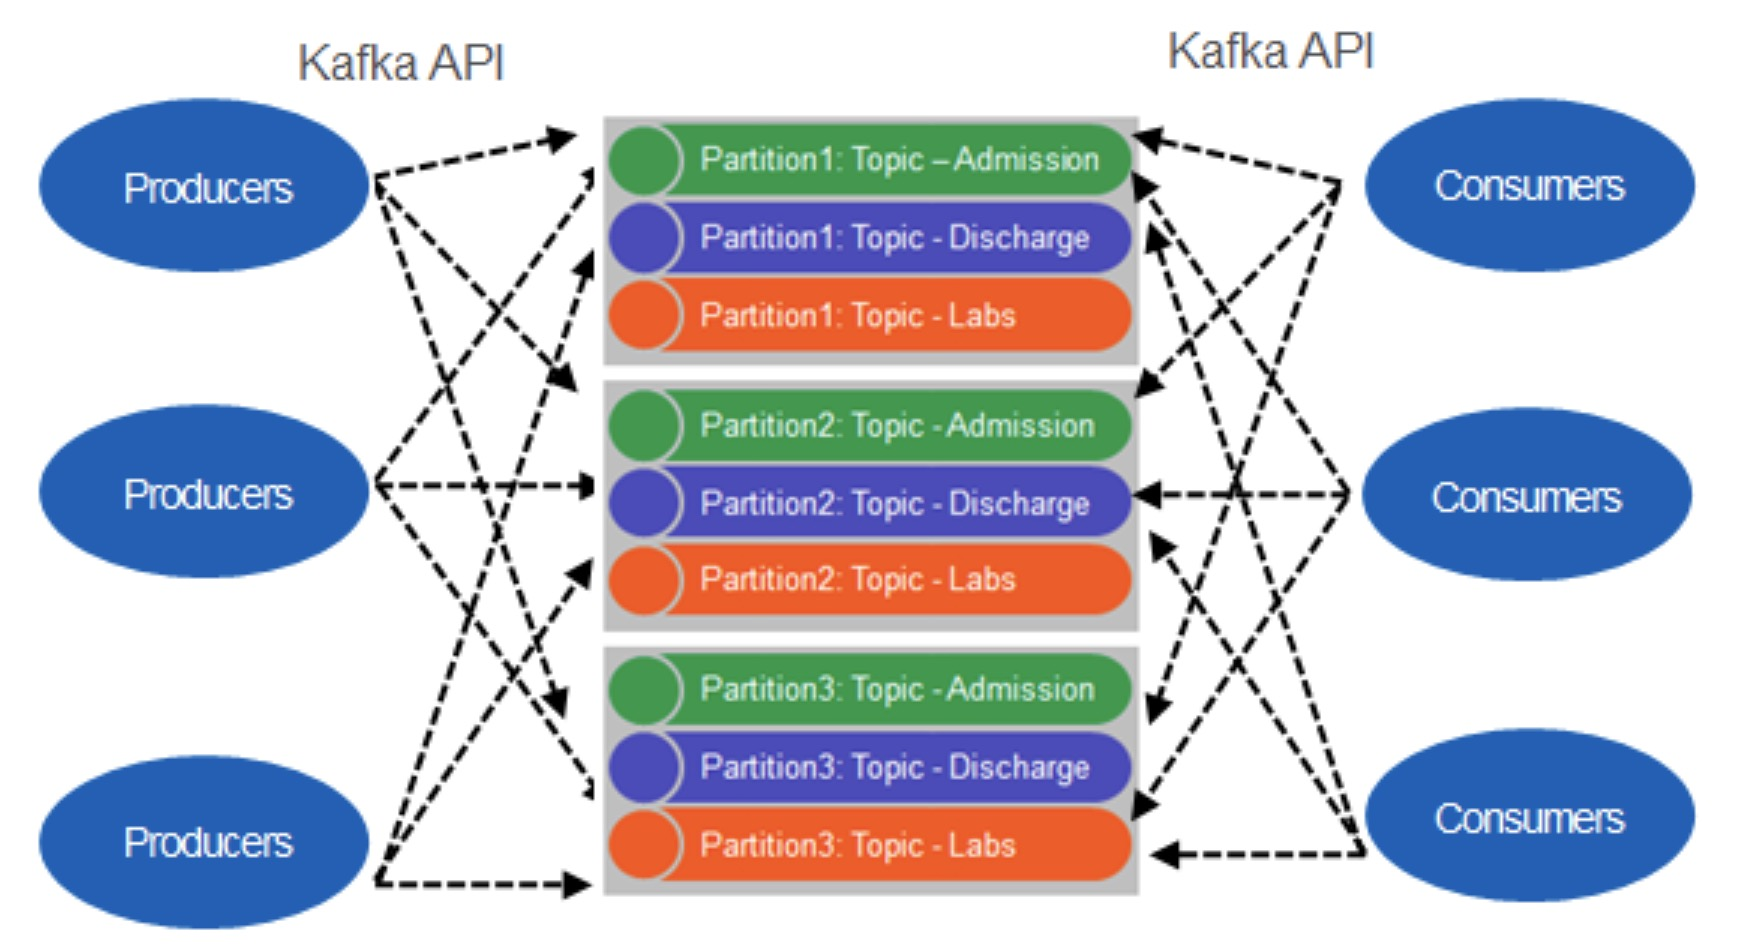
\includegraphics[width=\columnwidth]{images/mapr.png}
	\caption{The infrastructure of the MapR Stream}\label{f:mapr}
	\end{figure}
	
	\item Second Advantage - Partition Serves as a Similar 
	Function of Queue
	
Each partition offers similar functions with a queue as shown in  
Figure 3~\cite{stream}:

\begin{figure}[!ht]
	\centering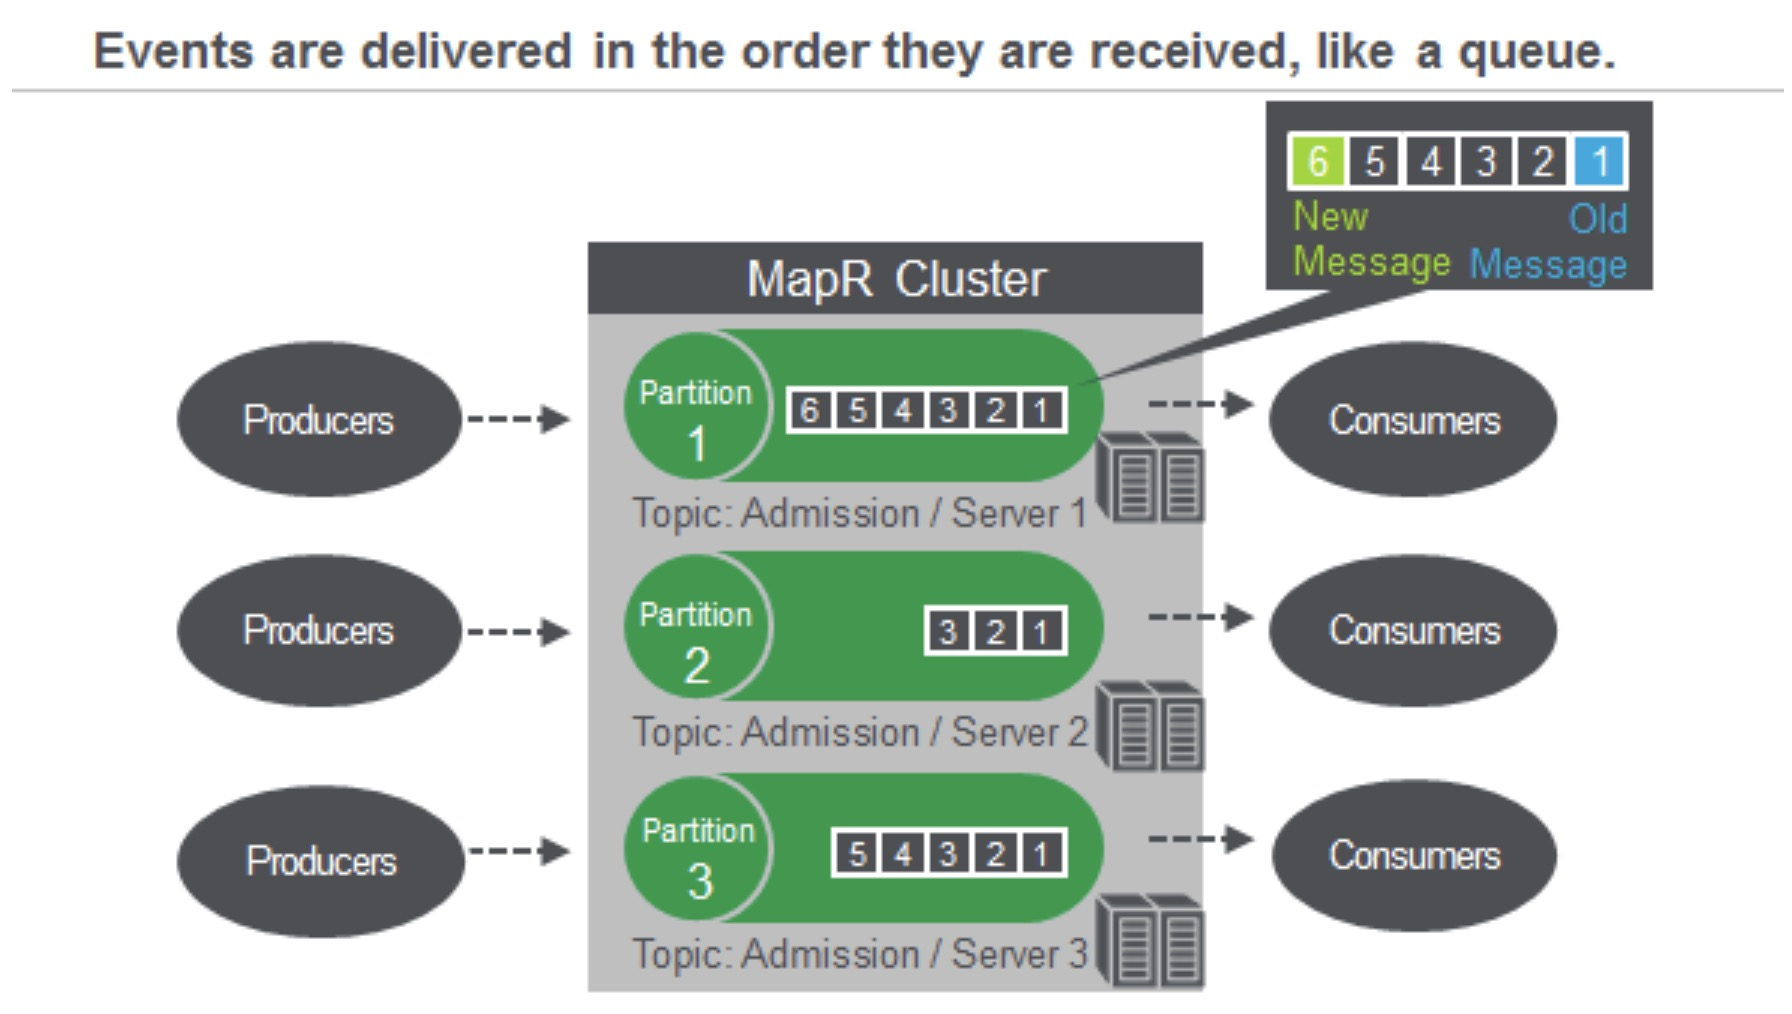
\includegraphics[width=\columnwidth]{images/mapr2.png}
	\caption{Partition Servers of the MapR Stream}\label{f:mapr2}
	\end{figure}

Messages with the specific topic will be appended 
to the corresponding partition 
and arranged in order according to the time they 
entered the partition 
(old messages with the high priority and a small 
number and new messages with
 the low priority and a big number). However, 
 data in the healthcare field is 
not only for one-time use, but it needs to be used 
multiple times. The point 
is that data needs to be delivered towards multiple 
destinations, unlike a queue,
so it will remain in the partition for a certain time to 
be accessible to
other users in the system. This feature provides an 
effective means 
of reusing and delivering data.

\end{itemize}

Other than MapR, there is another company 
called Liaison 
Technologies that uses the stream system to 
provide healthcare services. 
Liaison Technologies has 
become the leading company that uses this type of streaming 
technology for healthcare records.

Liaison uses its own platform called ALLOY to help 
customers analyze and transform data. Most of the time, 
a piece of a patient record needs to be observed 
in different formats, 
such as a graph, a document, or an 
analysis, and offered to various venues like clinics, 
hospitals, 
and pharmaceutical facilities. 
The ALLOY platform can transform this data in 
real time into 
various formats and update them 
to the cloud. More importantly, during the 
transformation process, the 
platform creates an analysis automatically 
based on its data analysis system, 
which provides customers the most useful 
information and helps 
them better understand the 
patient records, thereby helping the customers 
make the most 
correct decisions. 

Liaison Technologies is a company that provides cloud-based 
solutions to help 
organizations integrate, manage, and secure data across the 
enterprise~\cite{23}. One of the most widely used solutions 
they offer is to deal with 
health data in the healthcare 
and life sciences industry by using the MapR Stream system. 
With the implementation of MapR Stream, they have 
already solved two big difficulties of big data - the data and the 
system; it can meet 
HIPAA compliance requirements and the proliferation 
of data formats and representations~\cite{23}. 

\section{Future of Healthcare}
Today, the health care industry is driven by more and more 
medical data, and in
the future, the data will be even more complex, as the 
life science and medicine fields improve. As this paper mentions in 
Section 3, the data in the healthcare industry has not been stored 
in a uniform format, and the 
complexity of the health data is also another obstacle that 
complicates the data usage in the 
healthcare industry. Unfortunately, as the population on the 
earth grows, more and more health data will appear, 
with more complicated 
and potentially unusable data structures. It adds
more difficulties to using health data for analysis purposes. 
Furthermore, the cost
of collecting health data, maintaining integrity of the database, 
and correcting imperfect
data (such as missing and false values) will be greater. 
All of those trends apply to 
different healthcare systems, since the health data for people 
across the world is pretty much 
the same~\cite{f3,f4}.

Despite the idea that the data for healthcare fields will still be 
complicated and chaotic,the technologies in the distribution 
system, cloud computing, and the IoT will 
help remedy the shortage of usable health data. In the future, 
the distribution system used for healthcare service will includes 
multiple kinds of devices, such as wearable devices that collect 
the heath data directly from 
patients and update the data to the database directly. 
The IoT could be an 
important factor that helps remedy the 
imperfection of the health data by 
collecting the data in a uniform format 
(it depends on what the healthcare 
system needs), which significantly cuts 
the extra costs of collecting data 
and modifying that data~\cite{f2,f3}. 
The better the data quality is, 
the more precise dataanalysis results 
healthcare providers will have.

More that the health data, cloud computing, 
and IoT that serve the 
general public independently, in the future, 
hospitals could use 
these technologies together to build a concrete, 
multi-purpose 
healthcare service system. A hospital is a 
giant database that can 
collect the data directly from patients, so 
hospitals could collect 
data by themselves and then use them to 
design treatments for 
each patient, or use that data for research.
In the Mayo Clinic, in Minnesota, doctors could use 
health data to design special 
treatments for each patient and use 
advanced AI base 
study models to modify the treatment.
Additionally, the medical researchers 
from the Mayo Clinic use the health data 
from patients to study diseases, which 
accelerates the 
pace at which they can find methods of curing
certain diseases with firsthand data from 
patients~\cite{mayo}. 
In the future, the 
public and private hospitals could use 
the same mechanism of 
collecting and using data to provide better 
healthcare services to patients. 

In addition to the data and technologies 
changing the healthcare 
field today, the 
brain science field will also change the 
machine learning model in the future. 
As people learn more about the brain, 
a better study model will be created,
which helps the neural networks of 
some machine learning models to 
become more advanced. 
The improvement of brain science will give 
machine learning models a promising 
avenue for classifying 
and predicting jobs in every field, which also 
includes the healthcare 
field. Healthcare services or systems could use 
the more advanced 
study models to make decisions and create better 
health plans~\cite{brain}.

\section{Summary}
This paper talks about how Big Data shapes 
the healthcare field today, 
and it frames the health data as the 
fundamental element in the healthcare 
field, including how traditional 
data is different from the modern digital 
data and what issues in health 
data are still 
problematic. The summary of the health 
data that is used today has the 
following properties:
\begin{itemize}
	\item The health data will be more and 
	more predominantly digital. 
	The traditional health data will be 
	transferred to digital data with the digital 
	healthcare service growth.
	\item Data that is used in the healthcare field is complex, 
	and given that more health data will be added, 
	the volume and the complexity of data will make this health 
	data harder to use.
	\item The health data could be less 
	integrated due to many reasons: 
	for example, the 
	missing data could be caused by the patient being 
	unwilling to offer it because of the sensitivity 
	of the data or for security reasons.
\end{itemize}

Furthermore, the technologies related 
to the healthcare field and Big 
Data, such as IoT and cloud computing systems, 
have been introduced to provide better 
healthcare services. 
Those technologies help 
remedy the shortage of health data. 
For example, IoT could collect 
data directly from patients with a 
well-formed data format, which 
avoids creating missing data.
Additionally, the cloud computing 
systems and distribution system 
could be used for storing and
processing a massive amount of data. 
The development of Big Data technologies 
has brought the 
following improvements to the
health care field:
\begin{itemize}
	\item IoT: gives the possibility of collecting real-time 
	data directly from patients and 
	makes better use of the health data. 
	The real-time data updating might compromise
	patients' privacy, but for providing better services 
	and preventing emergency health 
	problems, this is a sufficient method. In the future, 
	the IoT devices will become more
	suitable for wearing.
	\item Cloud Computing and Distribution System:
	Cloud computing and distribution system offer 
	the computing power of collecting and
	 processing massive amount of data, which is 
	 supporting the current and future 
	 healthcare field. The learning model that used 
	 in the computing system is the core that 
	 helps people to make the rational healthcare plan.
\end{itemize}

In this paper, some instances of healthcare applications 
and companies are mentioned, 
those instances give people a great idea of how the 
healthcare services serve people 
from different aspects, for example, 
using data analysis to make healthcare plan, 
or predicting diseases from DNA and so on. 
Additionally, those instances are also provide people a more 
advanced ideas that how the 
healthcare should improved in the future.

In conclusion, the Big Data concepts and 
technologies will be applied more in the 
healthcare fields with advanced technologies, 
formatted database and IoT devices 
that gives people conveniences for planning 
their healthcare. The optimized views 
of healthcare comes from the massive investment 
on making data more meaningful 
to people. With the improvement in Big Data 
related technologies, the healthcare
fields will provide better services to people for 
maintain good health.
\section{Acknowledgments}
\begin{acks}

  The authors would like to thank Dr.~Gregor~von~Laszewski for his
  support and suggestions in writing this paper, as well as Nicole 
  DiPaolo for copyediting the final draft.

\end{acks}

\bibliographystyle{ACM-Reference-Format}
\bibliography{report} 

